\documentclass{ximera}
\input{../preamble}
\addPrintStyle{..}
\begin{document}
\author{Alexander Holvoet}
\xmtitle{Basis(sen) definiëren}{}

% Oefeningen: Coördinatentransformaties in ℝ²
% Gebaseerd op coordinate systems visualisatie

\begin{problem}
Beschouw de volgende twee coördinatenstelsels in $\mathbb{R}^2$: het zwarte coördinatenstelsel en het blauwe coördinatenstelsel. In de figuur zijn vijf punten aangeduid: $a$, $b$, $c$, $d$, en $e$.

\begin{center}
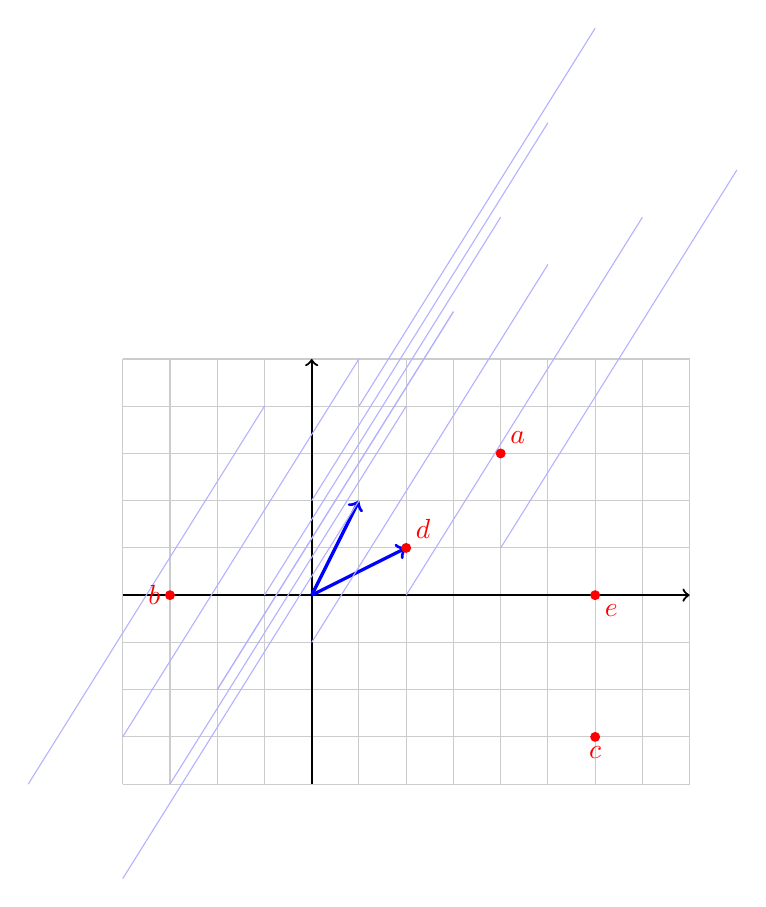
\begin{tikzpicture}[scale=0.6]
% Zwart coördinatenstelsel (standaard cartesiaans)
\draw[black!20, thin, step=1] (-4,-4) grid (8,5);
\draw[black, thick, ->] (-4,0) -- (8,0) node[right] {};
\draw[black, thick, ->] (0,-4) -- (0,5) node[above] {};

% Blauw coördinatenstelsel (geroteerd en geschaald)
% Blauwe basisvector 1: (2,1) in zwarte coördinaten
% Blauwe basisvector 2: (1,2) in zwarte coördinaten
\draw[blue, very thick, ->] (0,0) -- (2,1) node[midway, below right] {};
\draw[blue, very thick, ->] (0,0) -- (1,2) node[midway, above left] {};

% Blauwe rasterlijnen
\foreach \i in {-2,-1,0,1,2,3} {
  \draw[blue!30, thin] ({\i*2 - 2}, {\i*1 - 2}) -- ({\i*2 + 3}, {\i*1 + 6});
  \draw[blue!30, thin] ({\i*1 - 2}, {\i*2 - 2}) -- ({\i*1 + 3}, {\i*2 + 6});
}

% Punten
\fill[red] (4,3) circle (3pt) node[above right] {$a$};
\fill[red] (-3,0) circle (3pt) node[left] {$b$};
\fill[red] (6,-3) circle (3pt) node[below] {$c$};
\fill[red] (2,1) circle (3pt) node[above right] {$d$};
\fill[red] (6,0) circle (3pt) node[below right] {$e$};
\end{tikzpicture}
\end{center}

Schrijf de coördinaten van elk van de bovenstaande punten relatief ten opzichte van zowel het blauwe als het zwarte coördinatenstelsel.
\end{problem}

\begin{freeResponse}
Om de coördinaten te vinden, moeten we voor elk punt de afstand langs de basissen van beide coördinatenstelsels bepalen.

\textbf{Aanpak:} Gebruik de rasterlijnen om de componenten af te lezen in beide stelsels.

Uit de figuur lezen we (bij benadering):

\textbf{Punt a:}
\begin{itemize}
\item Zwart systeem: $(4, 3)$
\item Blauw systeem: $(2, 1)$
\end{itemize}

\textbf{Punt b:}
\begin{itemize}
\item Zwart systeem: $(-3, 0)$
\item Blauw systeem: $(-1, 2)$
\end{itemize}

\textbf{Punt c:}
\begin{itemize}
\item Zwart systeem: $(6, -3)$
\item Blauw systeem: $(3, -1)$
\end{itemize}

\textbf{Punt d:}
\begin{itemize}
\item Zwart systeem: $(2, 1)$
\item Blauw systeem: $(1, 0)$
\end{itemize}

\textbf{Punt e:}
\begin{itemize}
\item Zwart systeem: $(6, 0)$
\item Blauw systeem: $(3, 0)$
\end{itemize}

\textbf{Verificatie:} De punten die op een as liggen (zoals $e$ op de horizontale as) geven een nulcoördinaat in de andere richting.

\textbf{Mogelijke studentenfouten:}
\begin{itemize}
\item Verwarring over welke basis bij welk systeem hoort (basissen niet correct identificeren)
\item Verkeerde richting aflezen (mintekens verwisselen)
\item Vergeten dat de basissen verschillende lengtes kunnen hebben
\item De oorsprong van het blauwe systeem niet correct lokaliseren in het zwarte systeem
\end{itemize}
\end{freeResponse}

\begin{problem}
Bepaal een matrix die:
\begin{enumerate}
\item Punten van het blauwe coördinatenstelsel omzet naar punten in het zwarte coördinatenstelsel.
\item Punten van het zwarte coördinatenstelsel omzet naar punten in het blauwe coördinatenstelsel.
\end{enumerate}
\end{problem}

\begin{freeResponse}
\textbf{Conceptuele aanpak:} De transformatiematrix wordt gevormd door de basisvectoren van het ene systeem uit te drukken in het andere systeem.

\textbf{Deel a: Van blauw naar zwart}

We moeten de blauwe basisvectoren uitdrukken in zwarte coördinaten.

Uit de figuur zien we dat:
\begin{itemize}
\item De eerste blauwe basisvector (horizontale richting blauw) in zwarte coördinaten: $(2, 1)$
\item De tweede blauwe basisvector (verticale richting blauw) in zwarte coördinaten: $(1, 2)$
\end{itemize}

De transformatiematrix van blauw naar zwart is:
$$A_{b \to z} = \begin{pmatrix} 2 & 1 \\ 1 & 2 \end{pmatrix}$$

De kolommen zijn de blauwe basisvectoren uitgedrukt in het zwarte systeem.

\textbf{Verificatie met punt $a$:}
$$\begin{pmatrix} 2 & 1 \\ 1 & 2 \end{pmatrix} \begin{pmatrix} 2 \\ 1 \end{pmatrix} = \begin{pmatrix} 5 \\ 4 \end{pmatrix}$$

(Dit zou moeten kloppen met de zwarte coördinaten van punt $a$.)

\textbf{Deel b: Van zwart naar blauw}

Deze matrix is de inverse van de matrix hierboven:
$$A_{z \to b} = A_{b \to z}^{-1} = \begin{pmatrix} 2 & 1 \\ 1 & 2 \end{pmatrix}^{-1}$$

Bereken de inverse:
$$\det(A_{b \to z}) = 2 \cdot 2 - 1 \cdot 1 = 3$$

$$A_{z \to b} = \frac{1}{3} \begin{pmatrix} 2 & -1 \\ -1 & 2 \end{pmatrix} = \begin{pmatrix} 2/3 & -1/3 \\ -1/3 & 2/3 \end{pmatrix}$$

\textbf{Verificatie:} $A_{b \to z} \cdot A_{z \to b} = I$

\textbf{Mogelijke studentenfouten:}
\begin{itemize}
\item Rijen en kolommen verwisselen (basisvectoren als rijen schrijven in plaats van kolommen)
\item Vergeten dat de transformatie afhangt van de richting (blauw→zwart vs. zwart→blauw)
\item Verkeerde inverse berekenen (teken- of rekenfouten)
\item De basisvectoren verkeerd aflezen uit de figuur
\item Denken dat beide matrices hetzelfde zijn
\end{itemize}
\end{freeResponse}

\end{document}